%% ==============================
\chapter{Techniken der Dimensionsreduktion}
\label{ch:TechnikenDerDimRed}
%% ==============================


Hier werden ausgewählte traditionelle und moderne Techniken der Dimensionsreduktion vorgestellt.

\section{Traditionelle Methoden}
\label{ch:TechnikenDerDimRed:sec:TraditionelleMethoden}

Hier werden traditionelle Methoden vorgestellt.


\newpage

%% ==============================
\subsection{Principal Component Analysis}
\label{ch:TechnikenDerDimRed:sec:TradtionelleMethoden:subsec:PCA}
\nomenclature[Z]{PCA}{Principal Component Analysis}

%% ==============================
\subsection{Kernel Principal Component Analysis}
\label{ch:TechnikenDerDimRed:sec:TradtionelleMethoden:subsec:kPCA}
\nomenclature[Z]{kPCA}{Kernel Principal Component Analysis}

%% ==============================
\subsection{t-distributed Stochastic Neighborhood Embedding}
\label{ch:TechnikenDerDimRed:sec:TradtionelleMethoden:subsec:t-SNE}
\nomenclature[Z]{t-SNE}{t-distributed Stochastic Neighborhood Embedding}

\newpage

%% ==============================
%% ==============================
\section{Moderne Methoden}
\label{ch:TechnikenDerDimRed:sec:ModerneMethoden}
%% ==============================
Hier werden Moderne Methoden vorgestellt.

\subsection{Autoencoder}
\label{ch:TechnikenDerDimRed:sec:ModerneMethoden:subsec:AE}
\nomenclature[Z]{AE}{Autoencoder}

\begin{figure}[h]
	\label{fig:5-layer-Autoencoder}
	\begin{center}
		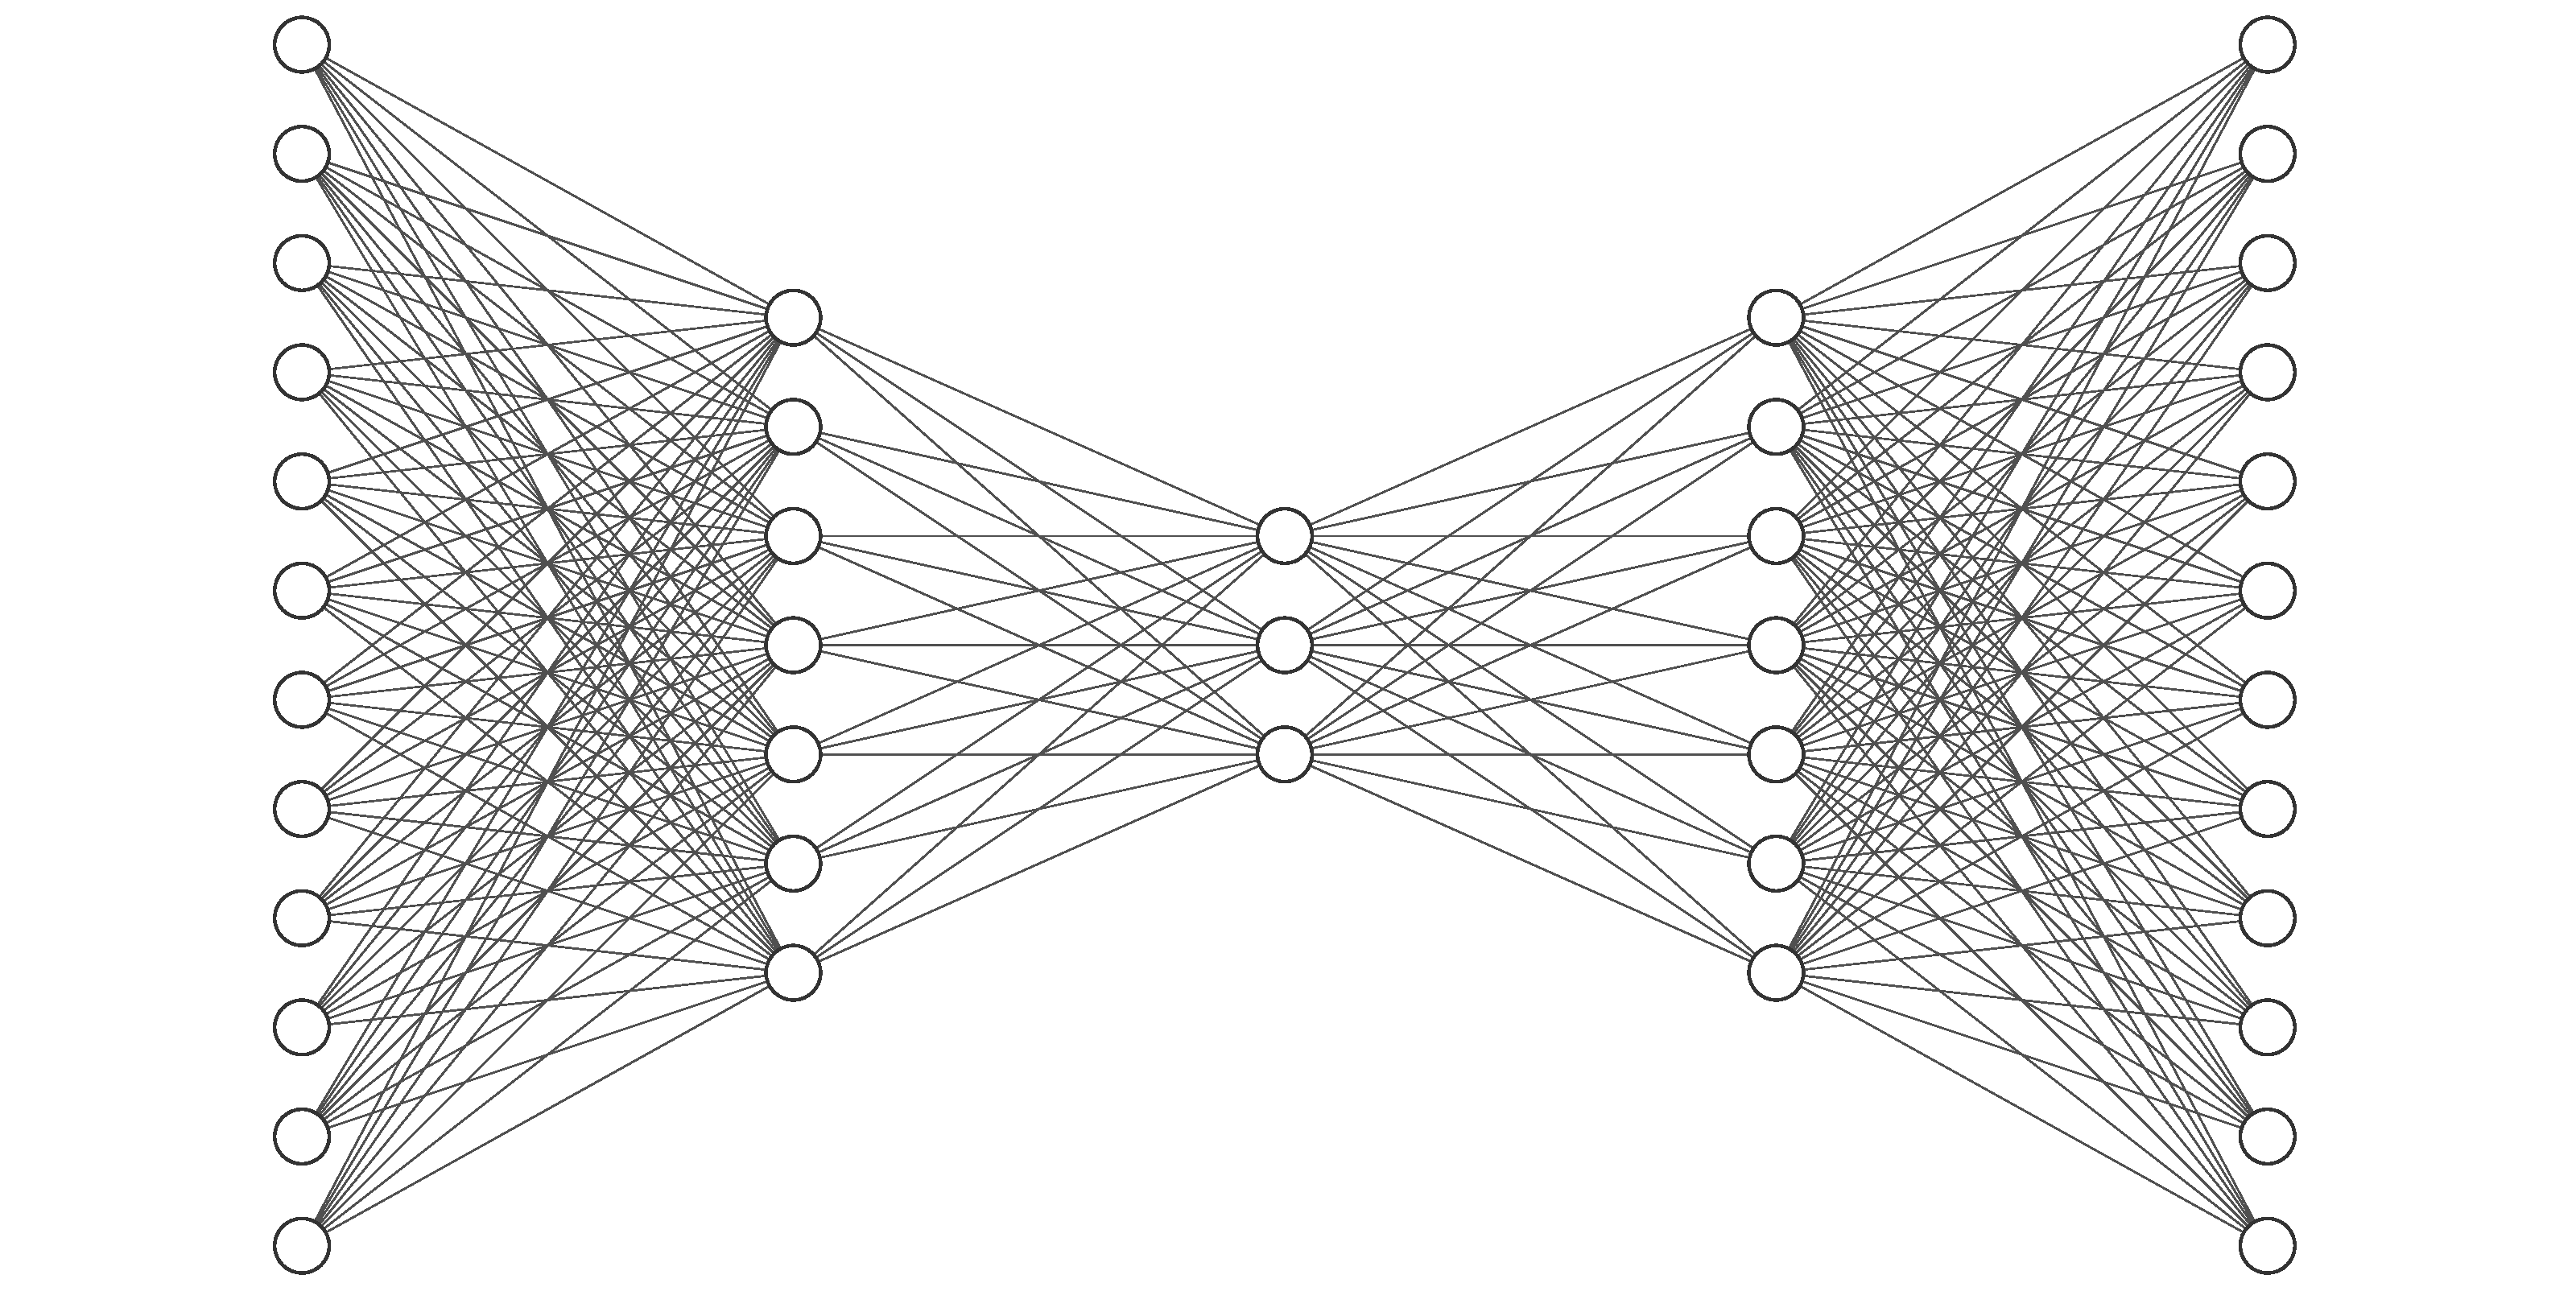
\includegraphics[width=\textwidth]{5_layer_AE.pdf}
		\caption{Autoencoder mit fünf Schichten und dreidimensionalem Bottleneck.}
	\end{center}
\end{figure}

\subsection{Variational Autoencoder}
\label{ch:TechnikenDerDimRed:sec:ModerneMethoden:subsec:VAE}
\nomenclature[Z]{VAE}{Variational Autoencoder}

\subsection{Self-Organizing Maps}
\label{ch:TechnikenDerDimRed:sec:ModerneMethoden:subsec:SOM}
\nomenclature[Z]{SOM}{Self-Organizing Map}
